%!TEX root = main.tex
%%%%%%%%%%%%%%%%%%%%%%%%%%%%%%%%%%%%%%%%%%%%%%%%%%%%%%%%%%%%%%%%%%%%%%%%%%%%%%%%%%%%%%%%%%%%%%%%%%%%%%
%
%   Filename    : chapter_4.tex 
%
%   Description : This file will contain your System Framework. About the system, pipline, use cases, anything that has to do with constructions and parts of the actual software/system. An overall look on the background of the system. Not sure which approach kung top down or reverse ba or some other way. Sorry fam.
%                 
%%%%%%%%%%%%%%%%%%%%%%%%%%%%%%%%%%%%%%%%%%%%%%%%%%%%%%%%%%%%%%%%%%%%%%%%%%%%%%%%%%%%%%%%%%%%%%%%%%%%%%

\chapter{Research Framework}

	%insert diagram here of the research framework
	\begin{figure}[H]
		\centering
		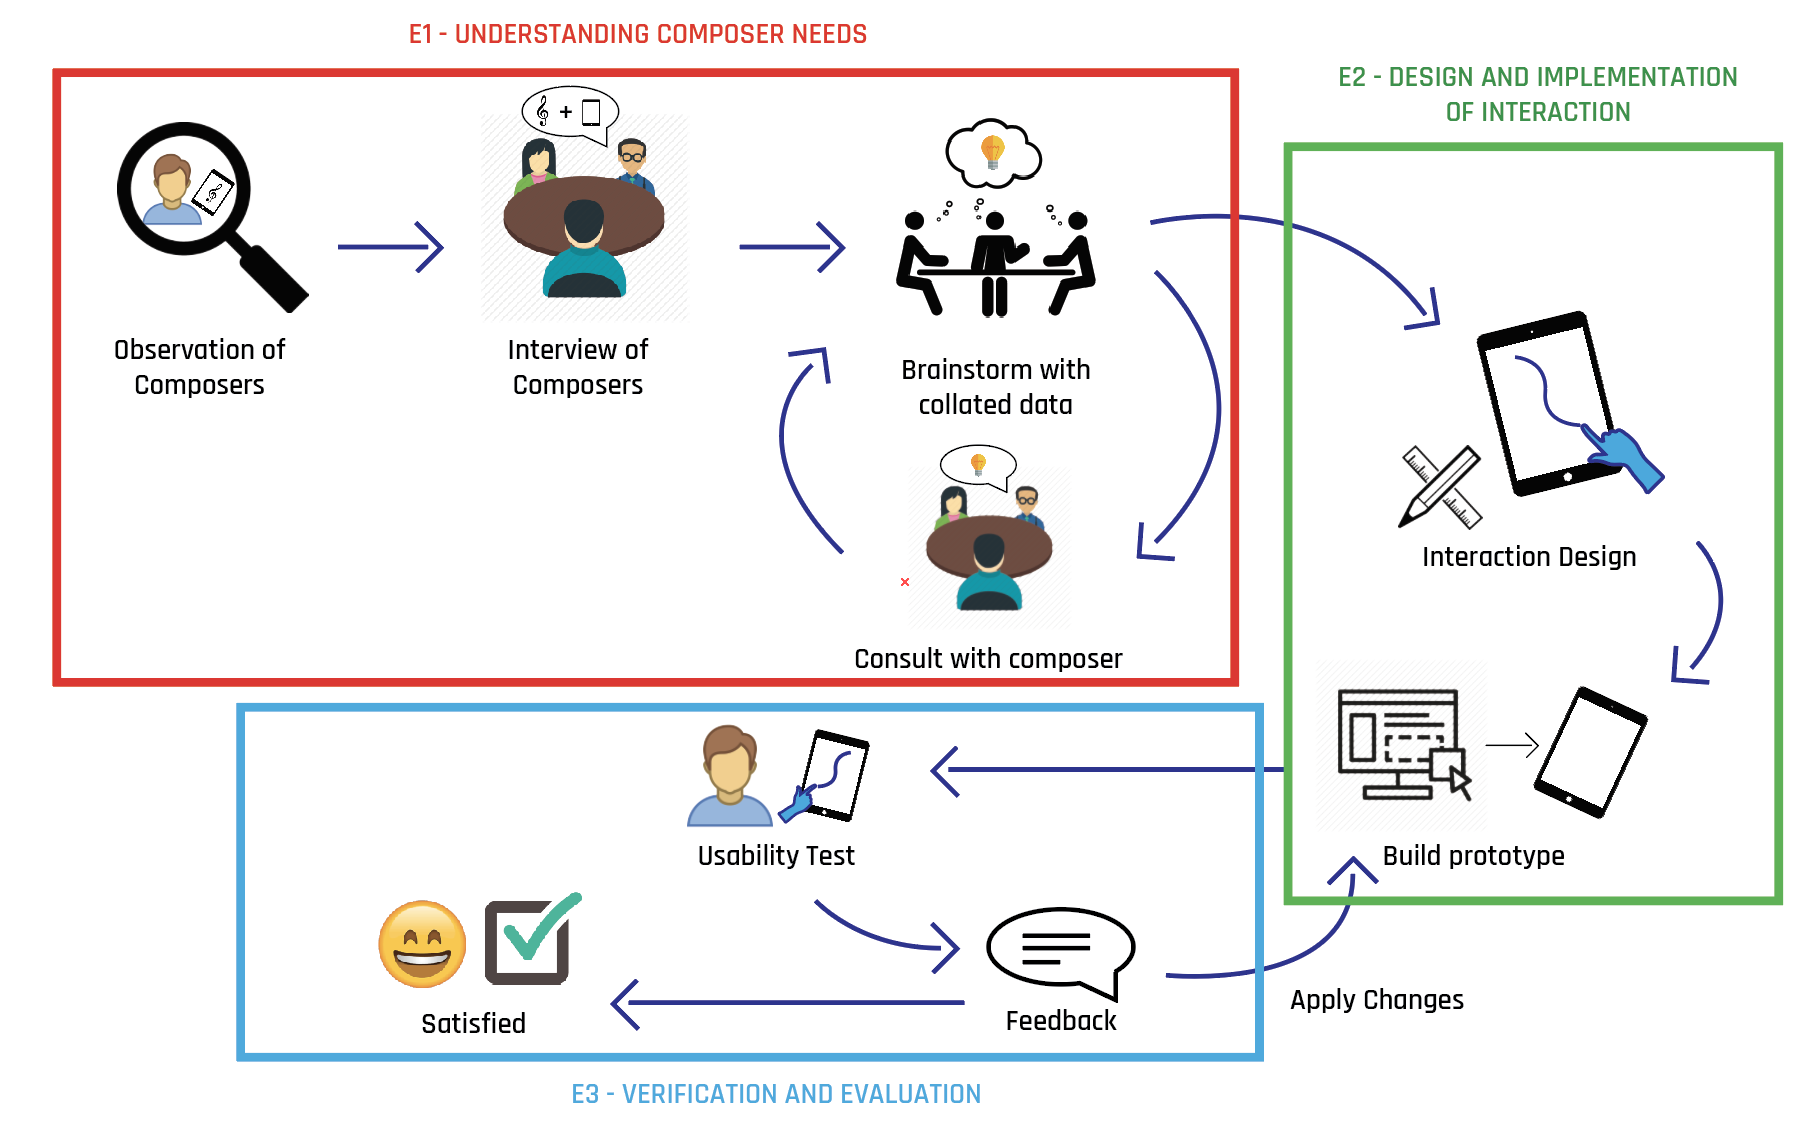
\includegraphics[scale=0.42]{figures/research_framework_sectioned.png}
	    \caption{The research framework for Flow.}
	    \label{fig:research_framework}
	\end{figure}

	The methodology for this study can be divided into three (3) main phases. The goal of the first phase (see Figure \ref{fig:research_framework} E1), is to understand the composers and identify their needs and problems. Using the gathered insights from the first phase, the second phase (see Figure \ref{fig:research_framework} E2)  will involve designing the interaction of the proposed solution. The last phase (see Figure \ref{fig:research_framework} E3) would then be an iterative process of testing and developing the proposed solution.


	\begin{comment}
	The goal of the first phase, \textit{understanding composer needs}, is to get to know more about the user and figure out their needs and pain points. User research and observation are key activities in this phase and is followed by interviews with composers to confirm and process the information as well as gather more insights. The points that were given by the composers would then be used in the brainstorming phase to determine a suitable solution. Consultations with composers will then be done to gather their insights on the proposed solution. This process will be repeated until the team is satisfied with the proposed solution.

	The next phase, \textit{design and implementation of interaction}, 
	\end{comment}

	\begin{comment}
	This study was designed to be repetitive and iterative, to allow for continuous improvement of the system. User research and observation are important steps to understanding the behavior of users and figuring out their pain points. This is followed by interviews with composers to confirm and process the information gathered from user tests and interviews. The points that were given by the composers would then be used in the brainstorming phase to determine a suitable solution. The team will then consult with the researchers about the proposed solution to gather their insights about it. The brainstorming would then be repeated to improve on the solution followed by another consultation. This would be repeated until the team is satisfied with the solution.

	The next phase would involve designing the interaction of the proposed solution. This would be followed by the prototype phase where a prototype would be built, tested, and improved repeatedly. Usability tests would be performed with different prototypes to create a good user experience. This phase would be repeated multiple times until the researchers are satisfied with the results of the tests.
	\end{comment}

	\begin{comment}
		Why/goal of the activity
		How we did it
	\end{comment}

	\section{Observation of Composers}

		Observations of the composers while they are composing music are necessary to understand the underlying thoughts and processes behind it. By doing this, the researchers were able to understand the thought-process and actions that composers undergo when composing music. The goal of this activity was to gather initial findings on the needs or pain points that the composers might have while composing. 

		This activity was mainly done in the studio of the composers or any place where they normally compose. The presence of instruments or any other tools depends on the composer as long as it simulates their natural composition process. 


	\section{Interview of Composers}

		Interviews were done to confirm and process the information and insights gathered from the observations made in the previous activity. Aside from this, further questions were asked about their process of musical composition, the tools, and the techniques they use. The main purpose of this activity was to get further context on the composition process and identify aspects that might not have been covered by the observations. 

		The main questions asked in the interviews are: 
		\begin{enumerate}
			\item What is your process of musical composition? What do you usually do?
			\item What techniques do you use during musical composition?
			\item What tools do you use when composing?
			\item What features do you like or often use in the tools you use?
			\item What are the difficulties you encounter when composing music? 
		\end{enumerate}

		Note that these are only the main questions and not all of the questions. Different questions may have come up depending on how the composer would answer a question to gather more insights. 

	\section{Brainstorm with Collated Data}

		After the observations and interviews, it is necessary to filter and process the gathered data to identify the needs and pain points of the target users. These needs and problems would then be the main focus when thinking of proposed solutions. 

		This study employed an affinity diagram for brainstorming. The affinity diagram is simply a tool that groups data or findings based on their relationships. This is done by identifying key points, observations, or ideas from composers that stand out and writing them on sticky notes. These may be behaviors, activities, things they said, or problems they encountered while composing and the workarounds they did to fix the problem. After writing them out, the items are grouped based on their relationships to identify similar or recurring ideas or problems. The affinity diagram will help identify the problem statement to focus on.

		With the problem statement in mind, the researchers can then ideate possible solutions. Ideation sessions put no limit on the amount of ideas that were generated; the more ideas the better. The researchers then voted on the ideas they liked and also provided suggestions on how to improve it. 

	\section{Consult with Composer}

		When a possible solution was thought of in the brainstorming activity, this was then consulted with the composers, the people who would actually use the it. Feedback and suggestions were also be gathered from the consultations to help improve the proposed solution. This, along with the previous activity, were be repeated until both the composers and researchers were satisfied.

		The identified needs and problems of the composers resulted in the list of user stories shown in Appendix \ref{sec:user_stories}.

		\subsection{System Features}

			From the feedback and insights gathered from the interviews and brainstorming sessions, it was found that the application should at least have the following features: 
			\begin{itemize}
    			\item View, create, edit, and delete their own compositions
    			\item Set the key and time signature of their compositions
    			\item Highlight/select a note or a group of notes
             	\item Add, edit, and delete notes/rests 
              	\item Add, edit, and delete polyphonic notes (chords)
           		\item Transpose a note or group of notes
        		\item Add ties/slurs to notes
              	\item Add, remove, or change an accidental on a note or group of notes
              	\item Add or remove dots on a note or group of notes
              	\item Apply retrograde/inversion on a note or group of notes
              	\item Cut, copy, and paste a note/rest or a group of notes/rests
              	\item Undo/redo an action
              	\item Zoom in our zoom out of the interface
              	\item Change the tempo
              	\item Listen to or play their composition
          	\end{itemize}				

	\section{Interaction Design}

		Using the input given by the composers, concepts for the initial interaction design were first sketched out on paper. The researchers created multiple designs based on their own idea on how to solve the composers' problems. This was followed by meetings that talked about the sketched out designs and how they could be improved. Once a design was agreed upon by the whole group, it was then converted to a mid-fidelity prototype in InVision for quick testing with the composers. 

		The mid-fidelity prototype allowed the researchers to quickly test out initial designs with composers. Although the prototype could not fully capture the experience of using an application, it made it faster to test out designs for the basic core tasks of adding, editing, and deleting. 

		When the more advanced features and tasks needed to be tested, an actual iOS application was built to support advanced interactions. The four (4) iterations of development and testing used different versions of the application, with each one using feedback from the previous iteration for improvements. 

	\section{Build Prototype}

		The initial, mid-fidelity prototype was built using InVision, a prototyping tool. Note that this was nowhere near an actual application and only consisted of screenshots or ``screens'' where users can interact with using the limited gestures in InVision. Despite the limited interactions available, doing this was quicker than actually developing the application, making it better for the earlier stages of testing the interaction design. The mid-fidelity prototype allowed the researchers to test out initial interaction design decisions and easily make the necessary changes. 

		Once the initial interaction design became clearer and more defined, it needed to be tested on a better platform since InVision was only limited to images and could never capture the complete interaction of the actual application. A high-fidelity prototype was then built for iOS and the iPad using Swift 4. This prototype went through four (4) versions, having changes in the interaction and the user interface. 

	\section{Usability Test}

		The objective of the tests were to determine if the interaction and design of the system augments the user experience of the composer when interacting with the application, Flow.  Quantitative and qualitative data were collected from the tests. The quantitative data mainly came from a survey about the usability of the features that the testers will have to answer. The qualitative data came from the video and audio recording of the testers as well as the interviews done after the tests. %The functionality was also closely monitored to see if there were glitches or bugs that required additional fixes in the development side. These bugs or glitches will warrant an intervention from the researchers during the testing. 

		The tests were conducted in an environment where audio and visual disturbances are at a minimum. This was to ensure that the researchers were able to analyze clear audio and video data from the recording devices used during the testing. This was also to ensure that distractions for the tester was kept at a minimum.

		%The setups used across all the user tests are 4 kinds of Flow system prototypes, 1 created using a prototyping tool called InVision, and 3 coded in Swift; 2 kinds of commercially available notation applications in the App Store, Notion and Komp; and the traditional form of composition which is using music sheets and writing materials. Notation softwares and the Flow prototypes will be launched on a mobile platform, namely an IPad tablet.

		Before starting the test, testers were given a consent form. If they agreed with the terms and continued with the testing, they were given a brief description of the objectives of the study along with overview of the tasks or use cases. The testers were asked to perform the tasks indicated in Section \ref{sec:tasks} for each test setup (indicated in Section \ref{sec:test-setups}) that is appropriate. 
		
		Composers of both genders aged 18-40 were recruited through snowball sampling method to take part in the data collection and testing. These subjects were categorized into two (2) user groups based on musical composition experience: amateur, and experienced. Iteration 1 and 2 had the same five (5) testers, made up of four (4) amateurs and one (1) expert. Iteration 3 had the most number of testers, having nine (9) amateurs and six (6) experts, for a total of fifteen (15) testers. Iteration 4 had three (3) amateurs and eight (8) experts totaling to eleven (11) testers, making it the iteration with the most number of experts. 

		\subsection{Test Setups}
		\label{sec:test-setups}

			The setups between the preliminary testing and the subsequent testing were different. This was made so because the main goal of the preliminary testing was to gather feedback on the interaction design and help improve the system while it was still being developed. Other applications did not matter as much and were only used to gain insight on their interactions and how they could be used to improve the system. Although the goal of the subsequent tests were still to gather feedback and improve the system, they were also made to compare the system against similar musical composition applications. 

			\subsubsection{Preliminary Testing Setups}

				The test setups are meant to observe how existing methods of composition work and how their interactions could be used in Flow. The tasks enumerated in Section \ref{sec:preliminary-tasks} will be used in each test setup whenever possible since some tasks can only be accomplished within a specific setup. 

				There will be 3 different test setups to be used during user testing namely:

				\begin{itemize}
					\item Tester composing using music sheets
					\item Tester composing using Komp
					\item Tester composing using Flow
				\end{itemize}

				The first setup simulates the traditional way of musical composition. This is through music sheets and a writing instrument. Traditional music sheets will be provided by the researchers as well as a choice of using a pen or pencil for writing musical elements. The composers are free to use as much music sheets as they want for drafting and experimenting with their composition as long as the time and resources provided by the researchers allow them.

				The second setup will be through an existing mobile application for iOS platforms, komp. Since the method of input in komp is similar to writing in music sheets, this setup will mainly be done to see how the interaction for traditional musical composition will work when applied to mobile devices. The researchers expect this setup to have similar results with the first setup and any data collected in this setup will be used to evaluate Flow.

				The third setup will be focused on the composer using the developed system, Flow. During the early periods of testing, a mid-fidelity InVision prototype will be used as a substitute. Using this prototype, the only task that the composer will be able to do is to explore the application. The main goal of this is to develop and improve the interaction design of the application. One a high-fidelity prototype has been developed, all tasks will be performed in the testing.

			\subsubsection{Subsequent Testing Setups}

				In the subsequent tests, Flow was compared against other musical notation applications. For each setup, the users had to go through the use cases listed in \ref{sec:use-cases} and perform the tasks outlined in \ref{sec:subsequent-tasks}. Note that these setups were given in random order and that the application developed by the researchers was not disclosed to prevent bias.

				\begin{itemize}
					\item Tester composing using Notion
					\item Tester composing using komp
					\item Tester composing using Flow
				\end{itemize}

				The first setup makes use of what is said to be the most popular musical notation application for mobile. For the second setup, komp is retained from the preliminary testing so that users can experience a traditional method of notation while on the iPad. The last setup makes use of the system developed by the researchers.

			\subsubsection{Use Cases}
			\label{sec:use-cases}

				For the subsequent test setups, the testers had to go perform use cases. These use cases were an attempt to simulate different musical composition scenarios. 

				\begin{itemize}
				    \item Compose a familiar song (Twinkle Twinkle Little Star/Happy Birthday)
				    \item Compose from scratch
				    \item Modify a composition (Ode to Joy/Amazing Grace)
				\end{itemize}

		\subsection{Tasks}
		\label{sec:tasks}

			Similar to the test setups, the tasks differed greatly between the preliminary testing and subsequent testing. Tasks were generalized in the subsequent testing to make it easier for the testers to compare the different applications.

			\subsubsection{Preliminary Testing Tasks}
			\label{sec:preliminary-tasks}

				Some tasks may be omitted in different test setups when a crucial function to carry out the task is unavailable. During the final task, testers are encouraged to speak aloud their concerns and opinions regarding the application.

				For the first iteration, there will be 4 tasks for each of the setups:
				\begin{itemize}
					\item Add a note
					\item Add a series of notes
					\item Change a note
					\item Delete/remove a series of Notes
					\item Compose for 3 minutes
				\end{itemize}

				For the second iteration, there will be 7 tasks for each of the setups:
				\begin{outline}
					\1 Add notes to fill 2 measures
					\1 Change the time signature to 3/4
					\1 Empty one measure
					\1 Empty the composition
					\1 Add enough notes to fill 2 measures in 2 staffs
					\1 Add an accidental to 2 notes
					\1 Remove placed accidentals 
					\1 Change key signature
					\1 Replace a group of notes with a single note
					\1 Create or recreate a composition (Exactly 4 measures)
						\2 Twinkle Twinkle Little Star
						\2 Canon in D
						\2 Ode to Joy
				\end{outline}

			\subsubsection{Subsequent Testing Tasks}
			\label{sec:subsequent-tasks}

				Since one of the goals of the subsequent tests was to compare how the interaction was against similar applications, the tasks were greatly simplified and generalized. Testers were also allowed to perform the tasks in any order they wanted and as much repititions it took for them to get acquainted with the specific task or action. These tasks were repeated for each of the use cases mentioned in \ref{sec:use-cases}.

				\begin{itemize}
					\item Select/highlight notes/chords
				  	\item Add notes/chords
				  	\item Edit notes/chords
				  	\item Delete notes/chords
				  	\item Cut, copy, or paste notes/chords
				  	\item Undo/redo an action
				  	\item Play the composition
				\end{itemize}


	\section{Feedback}

		Feedback came in the form of qualitative and quantitative data. The qualitative data was gathered through video recordings and interviews. Cameras were set up to capture expressions and hand movements while the testers while using the application (see Figure \ref{fig:test_setup}). Interviews were done after the tests to validate observations and gather more feedback on how the user experience was for the testers. 

		\begin{figure}[H]
			\centering
			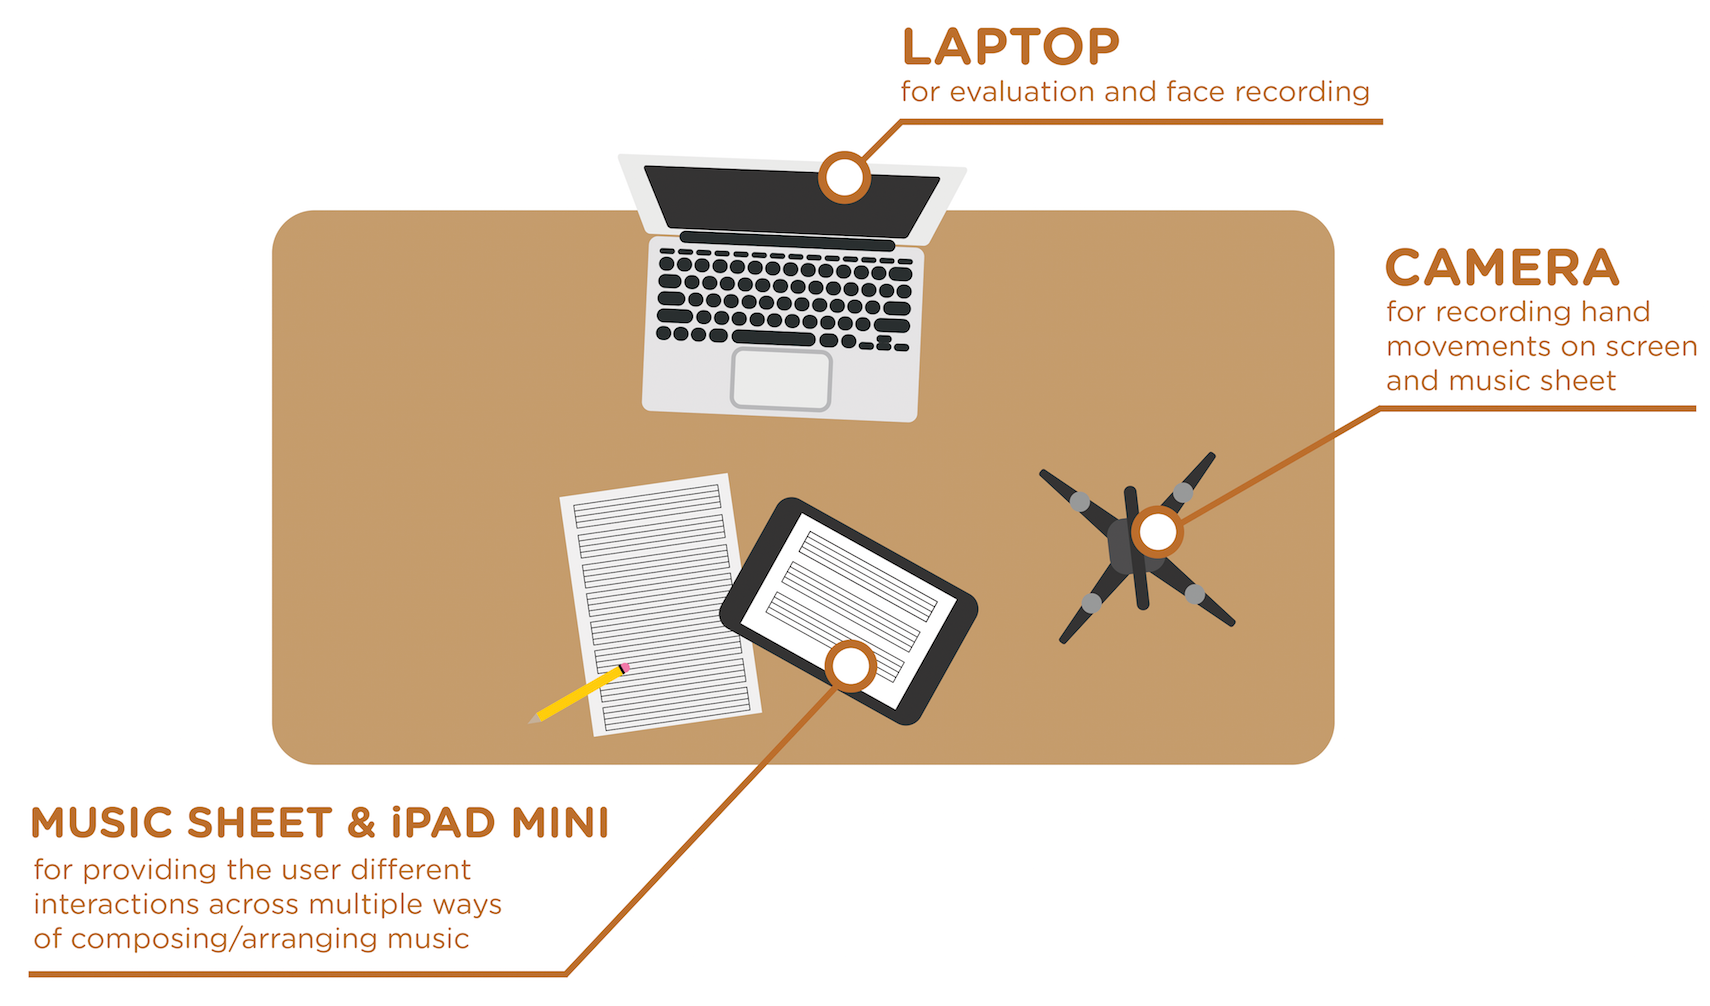
\includegraphics[scale=0.23]{figures/test_setup.png}
		    \caption{The standard setup for user tests.}
		    \label{fig:test_setup}
		\end{figure} 

		For each of the applications that were tested, the following questions were asked to understand more about the overall user experience and usability of the application and find any problematic features: 
		\begin{itemize}
			\item So why did you like/dislike \textit{$<$application$>$}?
			\item What did you feel while you were using \textit{$<$application$>$}? 
			\item What did you like most about \textit{$<$application$>$}? (Can be a feature, or the interface, or any part about it.)
			\item What did you least like about \textit{$<$application$>$}?
		\end{itemize} 
		
		\textit{If tester scored any features low in the questionnaire:}
		\begin{itemize}
			\item We noticed that you rated the \textit{$<$feature/s with low scores$>$} a bit low. Why is that?
		\end{itemize} 
		
		A typical interview would have the following format:
		\begin{outline}
			\1 Which of the three applications did you like using the most?
				\2 \textit{Ask questions for each application}
			\1 Which of the three did you least like using?
				\2 \textit{Ask questions for each application}
			\1 For the one in the middle…
				\2 \textit{Ask questions for each application}
		\1 Of the three applications, which one did you find the easiest to use?
			\2 Why?
			\2 On a scale of 1-4, with 4 being the highest, how usable is \textit{$<$application$>$}?
		\1 Which one did you find the hardest to use?
			\2 Why?
			\2 On a scale of 1-4, with 4 being the highest, how usable is \textit{$<$application$>$}?
		\1 And then lastly, the one in the middle…
			\2 Why?
			\2 On a scale of 1-4, with 4 being the highest, how usable is \textit{$<$application$>$}?
		\end{outline}
		
		On the other hand, quantitative data was collected through questionnaires. They were used to gather usability data on the different features of the applications, and easily identify problematic features. Note that iteration 1 and 2 used a different set of questions versus that of Iteration 3 and 4, because the main goal of iteration 1 and 2 was to improve the developed application while the main goal of iteration 3 and 4 was to compare applications. Answers to the questions were on a scale of 1 - 4, 1 (Never, Strongly Disagree, or Very Difficult) being the lowest, and 4 (Frequently, Strongly Agree, or Very Easy) being the highest. 

		Iteration 1 asked the following questions per feature: 
		\begin{outline}
			\1 How much did you use this feature to accomplish the tasks?
			\1 Were you comfortable while using this feature?
			\1 This feature feels like how I naturally \textit{$<$task$>$} when I’m composing.
			\1 This feature is new but easy to learn given enough time.
			\1 This feature makes the task at hand way easier than how I do things.
			\1 Is there any need to improve this feature? Why? (Optional)
		\end{outline}

		Iteration 2 used the same questions as that of iteration 1, but formatted to sound like sentiments: 
		\begin{outline}
			\1 I frequently used the \textit{$<$feature$>$} to accomplish tasks.
			\1 I felt comfortable using this feature.
			\1 This feature feels like how I naturally \textit{$<$task$>$} when I'm composing.
			\1 This feature is new but easy to learn given enough time.
			\1 This feature makes the task at hand easier than how I do things.
			\1 Is there any need to improve this feature? Why? (Optional)	
		\end{outline}

		In iteration 3 and 4, each feature only asked one question: 
			\begin{outline}
				\1 How easy was this activity to perform?
			\end{outline}

		With the exception of the music playback feature, which asked:
			\begin{outline}
				\1 How would you rate the music playback? 
			\end{outline}	
\begin{comment}
% \section{System Architecture and Framework}
\section{System Description}

\subsection{System Overview}

The system will integrate music theory and user experience in an interface for musical composition. The composition process of composers will be observed and analyzed so that the system can be built to fit this process. The system will undergo multiple revisions based on the results of user testing. It will be built for the iOS, but will be optimized for the iPad. It will provide users an interface to create/edit, and view compositions. The user can make use of the system through an interface containing compositional activities like adding, editing, and deleting notes. Finally, the system will allow users to save their composition, which can be imported to a MusicXML format.

\subsection{System Objectives}

	\subsubsection{General Objective}
		
        To provide an interface that allows composers to perform basic and advanced musical composition tasks via gesture interactions on a mobile platform.

	\subsubsection{System Features}
    
    	Specifically, the system will allow users to do the following: 
    		\begin{enumerate}
    			\item View, create, edit, and delete their own compositions
    			\item Set the key and time signature of their compositions
    			\item Highlight/select a note or a group of notes
             	\item Add, edit, and delete notes/rests 
              	\item Add, edit, and delete polyphonic notes (chords)
           		\item Transpose a note or group of notes
        		\item Add ties/slurs to notes
              	\item Add, remove, or change an accidental on a note or group of notes
              	\item Add or remove dots on a note or group of notes
              	\item Apply retrograde/inversion on a note or group of notes
              	\item Cut, copy, and paste a note/rest or a group of notes/rests
              	\item Undo/redo an action
              	\item Zoom in our zoom out of the interface
              	\item Change the tempo
              	\item Listen to or play their composition
          \end{enumerate}
    
\subsection{Scope and Limitations of the System}

Given that the system is on a mobile platform, it would be limited in ability compared to that of desktop applications. This system aims to be a sketching application for composers that are on the go, or do not have their computers available. It will not contend with full-blown desktop musical composition applications like Finale or Sibelius.

Musical composition can be done for several kinds of instruments. However, the way music is composed varies from one instrument to another. With that said, the system will only support compositions for the piano. The system will also limit the musical notation symbols that can be used. The ones available for use are: 

\begin{itemize}
	\item Sixty-fourth note to whole note
    \item Sixty-fourth rest to whole rest
    \item Accidentals (sharp, flat, double-sharp)
\end{itemize}

Composers will also need to save their compositions in cases where they could not finish entirely and want to go back to it. A composition also has several elements which would be hard to model in databases. Thus, MusicXML will be used as the file format for saving data. This also makes it easy to transfer work from the system to other musical composition applications.

Gesture interactions are the main method of interaction within the system. Some gestures like tapping on the line need to be accurate and precise. To improve this precision, bigger screens will be needed. The iPad will be the best for this due to it having a large screen, yet still being portable. The testing will also be done on the iPad only.

Finally, the system's potential musical metacreation feature will need to have a model for generating the succeeding notes. To make it lightweight, the system will make use of a rule-based model similar to that of Computoser \citep{bozhanov2014computoser} and SuperWillow \citep{schulze2011music}. The model will take into account music theory for its rules.

\subsection{Data Design}

Given that musical compositions have a lot of elements which need to be stored as data, using relational databases for storage would prove to be inefficient and unintuitive \citep{hristidis2003efficient}. That is why the system would represent data through the use of MusicXML, which was also used in the SuperWillow system found in the study of \citeauthor{schulze2011music}.

MusicXML is a method of storing and representing digital sheet music through XML \citep{makemusic2017musicxml}. Because it is an Extensible Markup Language (XML), it follows a specific format that defines a logical structure \citep{bray1997extensible}, which in this case is a musical composition. The advantage of the MusicXML format is that it is used in several musical composition applications and can easily be shared between these applications \citep{makemusic2017musicxml}. Also, it can represent the most complicated aspects of musical notation like repeats, slurs, and more.

Shown in Table \ref{tab:musicxml} are the some of the commonly used elements and their respective descriptions in MusicXML.
 
\begin{longtable}{|p{3.6cm}|p{10cm}|} 
\caption{Commonly Used MusicXML Elements} \label{tab:musicxml} \\
\hline
       
       Element & Description \\ \hline
		
        \texttt{<score-partwise>} & Defines that the composition is divided into several parts, and these parts can have multiple measures. \\ \hline
        
        \texttt{<score-timewise>} & An alternative to the \texttt{<score-timewise>}, it defines the composition to have multiple measures where the measures can have many parts. \\ \hline

		\texttt{<part-list>} & Lists the parts of the composition. \\ \hline
        
        \texttt{<score-part>} & To be used as a child of \texttt{<part-list>}, this element adds a new part to the composition. Commonly supplied with the \texttt{id} attribute. \\ \hline
        
        \texttt{<part-name>} & A child of the \texttt{<score-part>} element, specifies the name of its parent part. \\ \hline
        
        \texttt{<attributes>} & Lists essential information in the composition such as the key, time signature, and clef. \\ \hline
        
        \texttt{<divisions>} &  Used in the production of sound. It works with the \texttt{<duration>} element to tell how many divisions per quarter note equal to the duration indicated. \\ \hline
        
        \texttt{<key>} & Denotes which key signature the composition is in and contains the \texttt{<fifths>} element. \\ \hline
        
        \texttt{<fifths>} & This element is derived from the circle of fifths and says how many sharps or flats the composition has. \\ \hline
        
        \texttt{<time>} & The time element contains information about the time signature which can be set using the \texttt{<beats>} and \texttt{<beat-type>} tags. \\ \hline
        
        \texttt{<beats>} & The numerator of the time signature. \\ \hline
        
        \texttt{<beat-type>} & The denominator of the time signature. \\ \hline
        
        \texttt{<clef>} & Tells the clef to be used in the composition through the \texttt{<sign>} and \texttt{<line>} tags. \\ \hline
        
        \texttt{<sign>} & Specifies the sign to be used for the clef.\\ \hline
        
        \texttt{<line>} & Specifies which line the set sign will start. \\ \hline
        
        \texttt{<note>} & Contains information inside that is needed to define a single note. \\ \hline
        
        \texttt{<pitch>} & Located inside the \texttt{<note>} element, it contains the \texttt{<step>} and \texttt{<octave>} elements that would indicate where the note would be placed. \\ \hline
        
        \texttt{<step>} & Indicates the pitch step. Must always be supplied in the \texttt{<pitch>} element. \\ \hline
        
        \texttt{<octave>} & Indicates the octave of the pitch. Also required. \\ \hline

        \texttt{<alter>} & An optional element in the \texttt{<pitch>} that indicates if the note has a sharp or flat. \\ \hline
        
        \texttt{<duration>} & Also an element inside the \texttt{<note>}, it works with the \texttt{<division>} element to denote what kind of note or sound it would play. \\ \hline
        
        \texttt{<type>} & Mainly serves to indicate how the note will be displayed or notated. \\ \hline


\end{longtable}

Whenever a user creates a composition and saves it in the application, a corresponding MusicXML will be generated and saved in the device's local storage. The MusicXML will be used to load the composition again, in case the user wants to edit or view it. 

\subsection{System Framework}

\begin{figure}[H]
	\centering
	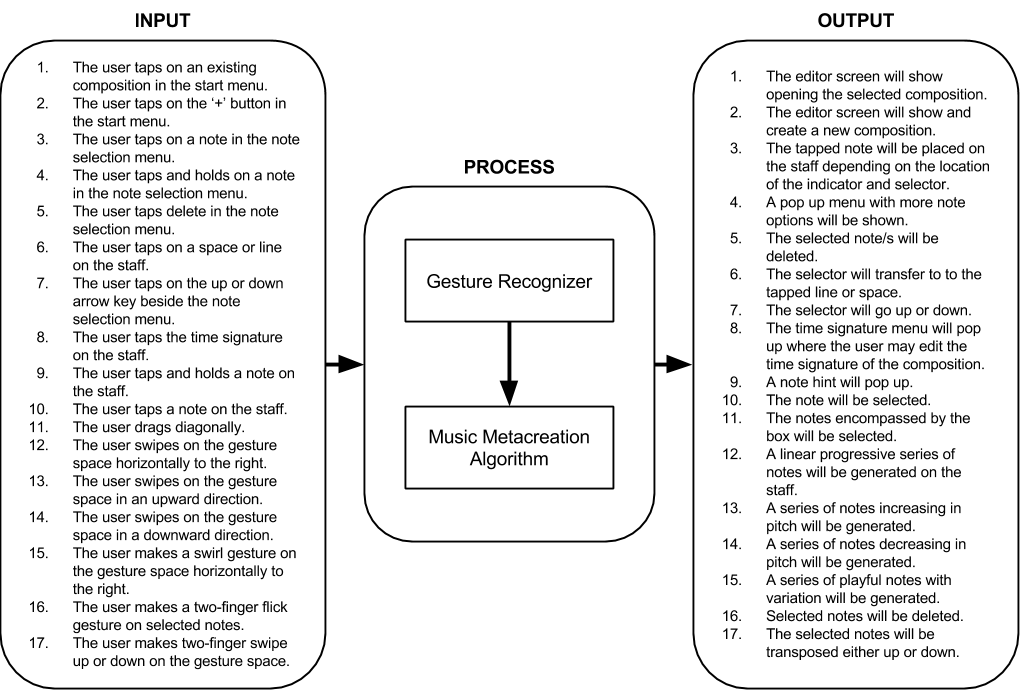
\includegraphics[scale=0.4]{System_Framework}
    \caption{The system framework for Flow.}
    \label{fig:systemframework}
\end{figure}

The system framework, shown in Figure \ref{fig:systemframework}, illustrates an overview of how Flow works. Input is relatively simple, mainly in the form of gestures. Users can tap, swipe, hold, or drag on specific objects. The application's gesture recognizer would then analyze the gesture performed by the user. The system would then output or perform the specific action assigned to each gesture. However, if the gesture is tied to musical metacreation, the application would output a set of notes based on its built-in algorithm.

\section{Experiment Design}

This chapter will describe the user stories and use cases that will be highlighted in the testing of the application. The intended users for the application will be expert composers who have at least 7 years of experience with composing music and amateur composers who have less than 7 years of experience composing music. These users should also have a basic knowledge of musical terms and are able to read and write musical notation. The details on the testing to be conducted on these users will also be discussed in this chapter.

\subsection{User Stories}
The user stories of the system will be focused on the main functions of the application and will highlight each specific need that the user has for the system. These user stories came from the users, representing the tasks that they need to perform on musical composition applications. These are created with the context that the system will run on a mobile platform with the mode of interaction mainly being touch gestures. 

\begin{enumerate}
\item As a user, I want to be able to create a blank composition, so that I can start my work
\item As a user, I want to be able to name my composition, so that I can differentiate it from my other compositions
\item As a user, I want to be able to save my composition, so that I can come back to it later
\item As a user, I want to be able to view all my saved compositions in a list, so that I can keep track of everything
\item As a user, I want to be able to open a saved composition so that I can perform more actions on it
\item As a user, I want to be able export my composition in a format that I can open in the composition application I use on my laptop
\item As a user, I want to be able to delete a composition, so I can discard compositions I do not work on anymore
\item As a user, I want to be able to add a chord progression in my composition, so that I do not need to individually add notes that belong to a progression
\item As a user, I want to be able to place a note in my composition, so that I can create my composition
\item As a user, I want to be able to select a single note, so that I can perform actions on it
\item As a user, I want to be able to change the pitch class of a note in my composition, so that I can make adjustments to my composition
\item As a user, I want to be able to change the type of a note in my composition, so that I can make the sound longer or shorter
\item As a user, I want to be able to erase a note in my composition, so that I can make space for other notes in my composition
\item As a user, I want to be able to highlight a group of notes in my composition, so that I can perform actions on the group
\item As a user, I want to be able to erase a highlighted group of notes in my composition, so that I can make space faster for other notes I'd like to place in my composition
\item As a user, I want to be able to place a rest in my composition, so I can have pauses in my composition
\item As a user, I want to be able to select a rest, so that I can perform actions on that rest
\item As a user, I want to be able to change the type of rest, so that I can change the length of pauses
\item As a user, I want to be able to highlight a group of rests, so that I can perform actions on the group of rests
\item As a user, I want to be able to erase a rest in my composition, so that I can make space for other rests or notes
\item As a user, I want to be able to change a rest in my composition, so that I can make adjustments to my composition
%\item As a user, I want to be able to move the position of a note in my composition, so that I can move that note to a better position
%\item As a user, I want to be able to move the position of a highlighted group of notes in my composition, so that I can reposition multiple notes at a time to a better position
\item As a user, I want to be able to hear the sound of the note I just added, so that I know I've added the correct sounding note
\item As a user, I want to be able to listen to a highlighted section of my composition, so that I can hear just a segment of my piece
\item As a user, I want to be able to listen to my whole composition, so that I can hear it as a whole
\item As a user, I want to be able to perform a swipe gesture that will generate a succession of notes based on the orientation of my gesture and my current composition because I'm interested in knowing what series of notes match my current composition
\item As a user, I want to be able to manipulate the generated series of notes, because the generated series of notes just needs a little bit more adjustments before I accept it into my composition
\item As a user, I want to be able to discard the series of notes generated by the application after a swipe gesture, so I do not have to delete them one by one
\item As a user, I want to be able to confirm the addition of the series of notes given by the application after a swipe gesture, so I can create my composition quickly
\item As a user I want to be able to undo an action or a series of actions, so that I can undo an unintended action or series of unintended actions quicker
\item As a user I want to be able to redo an action or a series of actions, so that I can redo an intended action or a series of intended actions quicker
\item As a user, I want to be able to reposition the menu because I want to place it where it is not an obstacle for me while composing
\item As a user, I want to be able to set the time signature of my composition
\item As a user, I want to be able to see the details of a single note, so that I can know the specifications of the note
\item As a user, I want to be able to see the details of a selected group of notes, so that I can know the specification of the selected group of notes
\item As a user, I want to be able to see the details of the generated series of notes like the pitch and type so that I can know what notes the system has generated after a gesture
\item As a user, I want to be able to set the clef of my composition
\item As a user, I want to be able to set the key signature of my composition
\item As a user, I want to be able to set the time signature of my composition
\item As a user, I want to be able to copy a highlighted group of notes and/or rests, so that I can copy a recurring segment in my composition
\item As a user, I want to be able to cut a highlighted group of notes and/or rests, so that I can copy a segment of my composition while at the same time making space for more notes
\item As a user, I want to be able to paste the copied or cut group of notes and/or rests onto my composition, so that I do not need to add a recurring segment in my composition manually all the time
%\item As a user, I want to be able to move the position of a rest, so that I can move that rest to a better position
%\item As a user, I want to be able to move the position of a selected group of rests, so that I can move multiple rests at a time to a better position
\item As a user, I want to be able to add accidentals to my notes, so that I can control the pitch of my notes
\item As a user, I want to be able to transpose a highlighted group of notes, so that I do not need to individually change the pitch of each note
\item As a user, I want to be able to perform retrograde inversion on a single note, so that I do not have to move it manually to invert it
\item As a user, I want to be able to perform retrograde inversion on a group of notes, so that I do not need to invert each note individually

\end{enumerate}

\subsection{User Test Plan}

The objective of the tests will be to determine if the interaction and design of the system augments the user experience of the composer while interacting with Flow. The functionality will also be closely monitored to see if there are glitches or bugs that require additional fixes in the development side. These bugs or glitches will warrant an intervention from the researchers during the testing.

The tests will be conducted in an environment where audio and visual disturbances are at a minimum. This is to ensure that the researchers are able to analyze clear audio and video data from the recording devices used during the testing. This is also to ensure that the tester is not disutbred during the testing. The setups used accross all the user tests are 4 kinds of Flow system prototpyes, 1 created using a prototyping tool called InVision, and 3 coded in Swift; 2 kinds of commercially available notation applications in the App Storem, Notion and Komp; and the traditional form of composition which is using music sheets and writing materials. Notation softwares and the Flow prototypes will be launched on a mobile platform, namely an IPad tablet.

Before starting the test, testers will be given a consent form. If they agree with the terms and continue with the testing, the tasks indicated in Section \ref{sec:tasks} will be done for each test setup (indicated in Section \ref{sec:test-setups}) that is appropriate. Before the start of the test where the tester start to accomplish tasks or use cases for the test setup, they will be given a brief description of the objectives of the study along with overview of the tasks or use cases. 

The researchers will be collecting quantitative and qualitative data. There will be tasks that the testers will be asked to accomplish, during iteration 1 and 2, after those tasks, data will be collected through an online form open after testing. During iteration 3 and 4, data will be collected during each use case through an online form. There will be video recording of the testers face and hand movements to be analyzed by the researchers during the testing. After the testing, for iteration 1 and 2, testers are then asked to answer a questionnaire to evaluate the quality of the application, and for iteration 3 and 4, testers are given a brief interview about their thoughts on each of the setups and the application.

During the first two (2) iterations, five (5) subjects of both genders aged 18-40 were recruited through snowball sampling method to take part in the data collection and testing. These subjects were categorized into two (2) user groups based on musical composition experience: amateur, and experienced. For the third iteration, fifteen (15) subjects of the same demographics took part in the testing. In the last iteration, ten (10) subjects took part. 

\subsection{Test Setups}
\label{sec:test-setups}

The setups between the preliminary testing and the subsequent testing were different. This was made so because the main goal of the preliminary testing was to gather feedback on the interaction design and help improve the system while it was still being developed. Other applications did not matter as much and were only used to gain insight on their interactions and how they could be used to improve the system. Although the goal of the subsequent tests were still to gather feedback and improve the system, they were also made to compare the system against similar musical composition applications. 

\subsubsection{Preliminary Testing Setups}

The test setups are meant to observe how existing methods of composition work and how their interactions could be used in Flow. The tasks enumerated in Section \ref{sec:preliminary-tasks} will be used in each test setup whenever possible since some tasks can only be accomplished within a specific setup. 

There will be 3 different test setups to be used during user testing namely:

\begin{enumerate}
\item Tester composing using music sheets
\item Tester composing using Komp
\item Tester composing using Flow
\end{enumerate}

The first setup simulates the traditional way of musical composition. This is through music sheets and a writing instrument. Traditional music sheets will be provided by the researchers as well as a choice of using a pen or pencil for writing musical elements. The composers are free to use as much music sheets as they want for drafting and experimenting with their composition as long as the time and resources provided by the researchers allow them.

The second setup will be through an existing mobile application for iOS platforms, komp. Since the method of input in komp is similar to writing in music sheets, this setup will mainly be done to see how the interaction for traditional musical composition will work when applied to mobile devices. The researchers expect this setup to have similar results with the first setup and any data collected in this setup will be used to evaluate Flow.

The third setup will be focused on the composer using the developed system, Flow. During the early periods of testing, a mid-fidelity InVision prototype will be used as a substitute. Using this prototype, the only task that the composer will be able to do is to explore the application. The main goal of this is to develop and improve the interaction design of the application. One a high-fidelity prototype has been developed, all tasks will be performed in the testing.

\subsubsection{Subsequent Testing Setups}

In the subsequent tests, Flow was compared against other musical notation applications. For each setup, the users had to go through the use cases listed in \ref{sec:use-cases} and perform the tasks outlined in \ref{sec:subsequent-tasks}. Note that these setups were given in random order and that the application developed by the researchers was not disclosed to prevent bias.

\begin{enumerate}
\item Tester composing using Notion
\item Tester composing using komp
\item Tester composing using Flow
\end{enumerate}

The first setup makes use of what is said to be the most popular musical notation application for mobile. For the second setup, komp is retained from the preliminary testing so that users can experience a traditional method of notation while on the iPad. The last setup makes use of the system developed by the researchers.

\subsubsection{Use Cases}
\label{sec:use-cases}

For the subsequent test setups, the testers had to go perform use cases. These use cases were an attempt to simulate different musical composition scenarios. 

\begin{enumerate}
    \item Compose a familiar song (Twinkle Twinkle Little Star/Happy Birthday)
    \item Compose from scratch
    \item Modify a composition (Ode to Joy/Amazing Grace)
\end{enumerate}

\subsection{Tasks}
\label{sec:tasks}

Similar to the test setups, the tasks differed greatly between the preliminary testing and subsequent testing. Tasks were generalized in the subsequent testing to make it easier for the testers to compare the different applications.

\subsubsection{Preliminary Testing Tasks}
\label{sec:preliminary-tasks}

Some tasks may be omitted in different test setups when a crucial function to carry out the task is unavailable. During the final task, testers are encouraged to speak aloud their concerns and opinions regarding the application.

For the first iteration, there will be 4 tasks for each of the setups with 1 special task for the setup using Flow:
\begin{enumerate}
\item Add a Note
\item Add a Series of Notes
\item Change a Note
\item Special Task - Delete a Series of Notes
\item Compose for 3 Minutes
\end{enumerate}

For the second iteration, there will be 7 tasks for each of the setups setups and 3 additional special tasks for the setup using Flow:
\begin{enumerate}
\item Add notes to fill 2 measures
\item Change Time Signature to 3/4
\item Special Task - Empty one measure
\item Special Task - Empty composition
\item Add enough notes to fill 2 measures in 2 staffs
\item Add an accidental to 2 notes
\item Remove placed accidentals 
\item Change Key Signature
\item Special Task - Replace a group of notes with a single note
\item Create or recreate a composition (Exactly 4 measures)
\subitem Twinkle Twinkle Little Star
\subitem Canon in D
\subitem Ode to Joy 
\end{enumerate}

\subsubsection{Subsequent Testing Tasks}
\label{sec:subsequent-tasks}

Since one of the goals of the subsequent tests was to compare how the interaction was against similar applications, the tasks were greatly simplified and generalized. Testers were also allowed to perform the tasks in any order they wanted and as much repititions it took for them to get acquainted with the specific task or action. These tasks were repeated for each of the use cases mentioned in \ref{sec:use-cases}.

\begin{enumerate}
  \item Select/highlight notes/chords
  \item Add notes/chords
  \item Edit notes/chords
  \item Delete notes/chords
  \item Cut, copy, or paste notes/chords
  \item Undo/redo an action
  \item Play the composition
\end{enumerate}
\end{comment}
